\begin{figure}
	\tikzsetnextfilename{intorno-d1-r2}
	\centering
	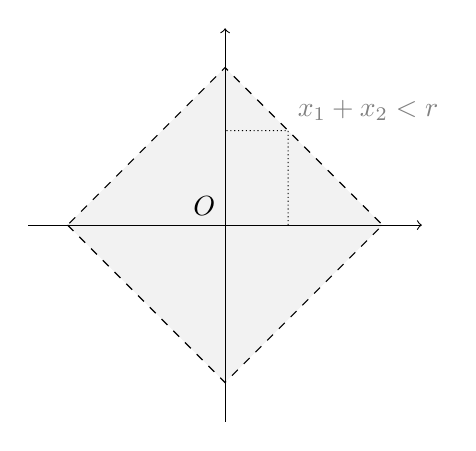
\begin{tikzpicture}
		\filldraw[dashed,fill=gray!10] (-2,0) -- (0,-2) -- (2,0) -- (0,2) -- (-2,0);
		\draw[->] (-2.5,0) -- (2.5,0);
		\draw[->] (0,-2.5) -- (0,2.5);
		\draw[densely dotted] (.8,0) -- (intersection of .8,0--.8,1 and 2,0--0,2) node[gray,anchor=south west]{$\abs{x_1}+\abs{x_2}<r$} -- +(-.8,0);
		\draw (0,0) node[anchor=south east]{$O$};
	\end{tikzpicture}
	\caption{Un intorno $B(\vec 0,r)\subset(\R^2,d_1)$.}
	\label{fig:B-d1}
\end{figure}
